\documentclass{article}
\usepackage{graphicx}
\usepackage{xcolor}
\usepackage[margin=3cm]{geometry} % margins might need to change in the future check with professor adam 
\setlength{\parindent}{0pt}
\usepackage{pgfgantt}


\begin{document}

\begin{center}
    \Large \textcolor{red}{\textbf{Electronics and Computer Science} \\[0.1cm]} 

    \large \textcolor{red}{Faculty of Engineering and Physical Sciences \\[0.1cm]} 

    \textcolor{red}{University of Southampton \\[1cm]} 

    \vspace{1cm} 

    \textcolor{red}{\textbf{\large Ashwinkrishna Azhagesh} \\[0.5cm]}

    \textbf{14/10/2024} \\[1cm] 

    \textbf{\large An AI Approach to Chaotic Physicl Systems: } \\[1cm]

    \vspace{0.5cm}

    Project supervisor: \textbf{Adam peugeot} \\[0.3cm] 
    Second examiner: \textbf{TBD} \\[1cm]

    Progress report submitted for the award of \\[0.1cm]

    \textbf{\large Bachelors of Science} 
\end{center}

\newpage

{\Huge \textbf{Abstract}}\\[1cm]

Physical laws are generalisation established through empirical observations
of the physical world. It has taken humans centuries to discover, requires huge
amounts of research, repeated experiments and plenty of scientists to produce
an universally accepted law in the scientific community. Thanks to recent
advances in neural networks and increased computational power, we can now
train models to replicate and fasten our discovery of physical laws such as the
laws of motion,also including chaotic systems such as the double pendulum,
drastically shortening the time required to find new physical laws. Furthermore
human’s have a cognitive bias when looking at data, find it difficult to spot
patterns in chaotic systems. This report explores how an AI without any bias or
prior knowledge views the physical world, how it is capable of spotting chaotic
patterns and how it is a tool that can reduce the time taken to make new
discoveries.\\

\newpage

\fbox{\underline{\textbf{Statement of Originality}}}
\\[0.5cm]

- I have read and understood the ECS Academic Integrity information and the University’s
Academic Integrity Guidance for Students.\\

- I am aware that failure to act in accordance with the Regulations Governing Academic Integrity
may lead to the imposition of penalties which, for the most serious cases, may include
termination of programme.\\

- I consent to the University copying and distributing any or all of my work in any form and
using third parties (who may be based outside the EU/EEA) to verify whether my work
contains plagiarised material, and for quality assurance purposes.\\

\fbox{
\underline{\textbf{You must change the statements in the boxes if you do not agree with them.}\\
}}
\\[0.5cm]

We expect you to acknowledge all sources of information (e.g. ideas, algorithms, data) using
citations. You must also put quotation marks around any sections of text that you have copied
without paraphrasing. If any figures or tables have been taken or modified from another source,
you must explain this in the caption and cite the original source.\\

\fbox{
\underline{\textbf{I have acknowledged all sources, and identified any content taken from elsewhere.}\\
}}
\\[0.5cm]

If you have used any code (e.g. open-source code), reference designs, or similar resources that
have been produced by anyone else, you must list them in the box below. In the report, you must
explain what was used and how it relates to the work you have done.\\


\fbox{
\underline{\textbf{I have not used any resources produced by anyone else.}\\
}}
\\[0.5cm]

You can consult with module teaching staff/demonstrators, but you should not show anyone else
your work (this includes uploading your work to publicly-accessible repositories e.g. Github, unless
expressly permitted by the module leader), or help them to do theirs. For individual assignments,
we expect you to work on your own. For group assignments, we expect that you work only with
your allocated group. You must get permission in writing from the module teaching staff before
you seek outside assistance, e.g. a proofreading service, and declare it here.\\

\fbox{
\underline{\textbf{I did all the work myself, or with my allocated group, and have not helped anyone else.}\\
} }
\\[0.5cm]

We expect that you have not fabricated, modified or distorted any data, evidence, references,
experimental results, or other material used or presented in the report. You must clearly describe
your experiments and how the results were obtained, and include all data, source code and/or
designs (either in the report, or submitted as a separate file) so that your results could be
reproduced.\\

\fbox{
\underline{\textbf{The material in the report is genuine, and I have included all my data/code/designs.}\\
}}
\\[0.5cm]

We expect that you have not previously submitted any part of this work for another assessment.
You must get permission in writing from the module teaching staff before re-using any of your
previously submitted work for this assessment.\\

\fbox{
\underline{\textbf{I have not submitted any part of this work for another assessment.}\\
}}
\\[0.5cm]

If your work involved research/studies (including surveys) on human participants, their cells or
data, or on animals, you must have been granted ethical approval before the work was carried
out, and any experiments must have followed these requirements. You must give details of this in
the report, and list the ethical approval reference number(s) in the box below.\\

\fbox{
\underline{\textbf{My work did not involve human participants, their cells or data, or animals.}\\
}}
\\[0.5cm]


ECS Statement of Originality Template, updated August 2018, Alex Weddell aiofficer@ecs.soton.ac.uk\\


\newpage 

\tableofcontents 



\newpage 

\section{Introduction: }

\subsection{Goals: }

It took humans centuries to derivie physical laws, can this process be sped up through AI, by feeding it data and letting the model derive complex laws for us. I aim to derive physical laws, from experimental data. I will explore deriving simpler physical laws such as acceleration without air resistance, and move onto to complex chaotic systems such as pendulums, and explore how an unbiased AI views the physical world, compared to humans who's views of physical systems are naturally biased through systematic learning. 

Can this lead to perhaps different prespectives of viewing the physical world around us, allowing for further progress? 


\subsection{Scope: }


 - Aim to derive simple laws of motions (ie acceleration) through AI frameworks.\\ 

- Move onto more complex systems such as pendulums, and initially explore smaller initial values, moving onto larger initial values, 
thereby increasing the chaos, and difficulty of spotting patterns. \\

- To explore using various AI techniques, (Graph Neural Networks, Deep learning, Neural Networks) in combination with no prior knowledge and observe how and in what form the physical laws are derived.  
- Simulate physical data required using pymunk, and perhaps use real world data from physics labs.\\ 

\section{Literature Review: }

\subsection{ Introduction: }
  
Humans have spent millennia observing the world around us, creating concepts that describe the variables in the physical world, such as mass and force, to derive the laws of motion. In physics, like with
all human endeavours, new discoveries and ways of thought are based upon previous works, creating
a natural bias in the way we humans approach new problems. All existing theories, are therefore
somewhat biased, this combined with our pre-existing bias in our biological brains, can introduce some
hurdles in our future progress [1,2].\\

In the 17th Century, Kepler had gotten his hands on the word’s most precise data tables on the orbits
on planets, using this and his intellect, he spent close to half a decade, and after numerous unsuccessful
attempts, he had began a scientific revolution at the time, describing Mar’s orbit to be an ellipse [3].
In essence, scientists throughout history, much like Kepler, have spent a great deal of time, discovering
the right expressions to match the relevant data they have, this at it’s core is symbolic regression. Now,
a few centuries later, with exponential increases in orders of magnitude in our capability to perform
calculations through computers, the process of discovering natural laws and the way to express them,
has to some extent resisted automation.\\


One of the core challenges of physics and artificial intelligence, is finding analytical relations automatically, discovering a symbolic expression that accurately matches the data from an unknown function.
This problem, due to it’s nature, is most certainly NP-hard [4] in principle. The vastness of the space
of mathematical constants, further adds to the difficulty. This literature review aims to present the recent advances in deriving expressions and laws through data, how we can avoid human bias by seeking
solutions without prior assumptions and describing the various tools and techniques used to achieve
this. Then it will introduce the 3-body problem and explore how artificial intelligence is being used to
6find faster and more efficient solutions.\\


\subsection{Symbolic Regression: }

Symbolic regression, is a technique that analyses and searches over the space of traceable mathematical
expressions to find the best fit for a data set. By not requiring prior information about the model,
it is unbiased. There are a plethora of various strategies that have been implemented in solving for
empirical laws [5], we will explore some of them below. It is also worth mentioning, that unlike other
well-known techniques for regression, (eg: neural networks), that are essentially black boxes, symbolic
regression, aims to extract white-box models and is easy to analyse.\\

\begin{center} 
  \textbf {\Large  Brute Force:}
\end{center}
Symbolic Regression (SR), is interpretable [6], unlike Neural Networks (NN), which are often considered more explainable. The difference is interpretability allows us to comprehend how the model works,
like observing how gears move in a glass box, while explainable means you get an overview of why a
certain output was achieved, even without knowing the full nuances of it’s inner workings.\\

There however, are some challenges associated with SR, in comparison to function fitting (NN). SR,
starts with nothing, a blank slate, and it has to learn the entire expression [7], unlike function fitting
which just tweaks an already existing function. The exponential search space [8] , causes it to be
extremely computationally expensive to explore all possibilities. This combined with the face that,
most optimisation algorithms expect a smooth search space [9], however SR lack’s smooth interpolation, small changes in the potential solutions (expression), ie: $ x3 and x3 + 0.1$ can significantly alter
the the output. Finally, if the nature of the problem is badly posed [10], there might potentially be
multiple solutions to the same data. Imagine trying to find a single polynomial equation with only two
points of data, the need to balance finding accurate expressions with finding the most simplistic and
generalisable fit, is sometimes troublesome.\\

The brute force approach of simply trying all possible combinations of symbolic expressions within some defined space. The model will subsequently increase the complexity over time, and will stop when either the fitting errors lowers below some defined limit or exceeds the upper limit of runtime. While in theory can solve all of our problems, in practise takes longer than the age of our universe to finish. In essence it's like searching for a singular drop in the ocean. Thankfully, there are some ways of pruning the search space, and drastically reducing the time taken to solve for the most accurate expression. \\ 

\begin{center} 
  \textbf {\Large Partial Derivatives:}
\end{center}

Partial derivatives, of some function f, with multiple variables such as x and y, is it's dervative with respect to one of those two variables, while the other variables in the function are kept constant. Formally, given a function with two or more variables, $f(x_1, x_2, \ldots, x_n) $, the partial derivative of $f$ with respect to $x_i$, where $x_i$ is some value $x$ in $(x_1, x_2, \ldots, x_i, \ldots, x_n)$, gives the rate of change of $f$ with respect to $x_i$. It is calculated by taking the ith derivative of $f$ with respect to $x_i$, whilst holding the other variables fixed. [11] \\

The partial derivative of a function $f(x,y)$ with respect to $x$ is denoted $\frac{\partial f}{\partial x}$ [12] and is defined: \\ 

\begin{center}

  $\frac{\partial f}{\partial x} = \lim_{h \to 0} \left[ \frac{f(x+h, y) - f(x,y)}{h} \right]$
\end{center}


Once you pass in the experimental data, you can pre-process the data, using calculated partial derivatives, for every pair of existing variables. Many physical laws, involve rates of change, and partial
derivatives help us represent them. Furthermore it also guides the search process, as the algorithm can
use the derivative to accurately represent the underlying laws involved. Through comparing how well
the partial derivatives derived through the experimental data compared to the potential expression,
the algorithm can assess the accuracy and feasibility of the expressions involved. This strategy can
even be extended to prune the search space further, this could be achieved through incorporating
knowledge of physics into the constraints for the partial derivatives. These concepts will be illustrated
with an example below.\\


Consider a iron rod, that has been heated up, such that it is hotter on one side than the other. Now it is intuitive to say that closer to the heat source, the temperature will be higher than further along the rod, where it will be colder. We can illustrate this temperature distribution with a function:  \\

\begin{center}
$T(x,y,z)$
\end{center}

where T is the temperature at a point in the rod, and (x,y,z) are the coordinates along the axis in 3 dimensions. This leads to these 3 partial derivatives: \\ 

\begin{center}
 $\frac{\partial T}{\partial x}, \  \frac{\partial T}{\partial y}, \  \frac{\partial T}{\partial z}$
\end{center}

These partial derivatives, gives us information about the direction and magnitude of heat flow at various points on the rod. The algorithm then searches for an equation T(x,y,z), that sufficiently predicts the observed temperature distribution and it's partial derivatives, deriving laws such as the heat transfer equations, or elasticity relationships.\\ 

\begin{center}
$\frac{\partial T}{\partial t} = \alpha \nabla^2 T$
\end{center}



Through using partial derivatives, we have in essence redefined the search criteria for the algorithm, through it's measure of the accuracy in comparison of potential solutions over the invariants represented in the experimental data [22] . This also leads to the pleasant finding, that it can additionally capture relationships that represent other identities of the system, beyond invariants and heat transfer equations. \\ 

You can subtly guide the type of laws that such an algorithm finds, by selectively picking the variables to input into the algorithm,. For example providing velocities and force to find laws of motion. \\ 

% THIS IS VERY BADLY WRITTEN! DOES NOT FLOW AT ALL\\ 


% some sort of analytical search method- “Distilling Free-Form Natural Laws from Experimental Data\\

% narrowing search space through explanable ai - From Kepler to Newton: Explainable AI for Science Discovery\\

\begin{center} 
  \textbf {\Large Dimensional Analysis:}
\end{center}

Dimensional Analysis is a method of solving problems usually in maths and physics, where we analyse
the relationships between different physical quantities, by comparing their ”units.” It is a powerful
method of reducing the complexity of systems, enabling engineers and scientists to analyse problems
that we can’t even pose, much less solve the equations of [13].\\

Using the fact that numerous questions in science can be simplified by requiring the dimensions/units
of the right and left hand side of the expression to be equal, we can transform the question into
a smaller number of variables, which all have no dimension [21]. It has been automated to find the integer powers of expressions and has proven to be useful especially when the power is an irrational number.\\

Here is a general strategy that showcases how dimensional analysis can be used:\\

Let's say we have a variable in an equation that can be broken down into it's fundamental units, such as (second, kilograms, ampere ...) to various powers. We can then take this, and represent each of the units as vectors, such that each of the fundamental units, is assigned a dimension, and it's important to note, this then allows us to represent any physical quantity as a product of these units, so let us construct a vector $v$, with $3$ integers, where each corresponding integer represents the power of each of the fundamental units.\\ 

Given that we want to derive an expression, such as $y = f(x_1, \dots, x_n)$  we can then create some matrix $M$. Each of the columns of the given matrix, is the unit vector $v$ of the corresponding variable $x_i$. We then need to define another vector to represent the units of y, which will be called $z$. If we let the solution be some vector $s$, solving $Ms = z$, this then lets us raise the powers on both sides, to elevate the independent variables, to make this equation dimensionally consistent.\\ 

Taking the null space of the matrix $M$, where $MV = 0$, allows us a basis to create a dimensionless group, allows for a simplification of the problem.\\

This is also more intuitive to understand physical phenomena, the nature of physics comprehension, making this vital in further understanding derived laws, making the process easier to explain and understand [14,15]. Therefore, this is a crucial tool, for cultivating a deeper understanding of physics effectively [16]. \\






\begin{center} 
  \textbf {\Large Genetic Programming:}
\end{center}


Genetic programming (GP), is a special evolutionary algorithmic technique, where the individuals are seen as programs that evolve, starting for a population, is iteratively "evolved," transforming the populations of individual programs, intro other populations. This new generation of programs are created using some genetic operations or survival criteria, mimicking natural evolutionary condition on earth.\\ 

A very basic overview, shows that genetic programming algorithms, consists of initializing the population, then evaluation of the said population through some predefined metrics and functions, followed by selection of the fittest programs based on the score given by the metric, and "genetic operation," such as reproduction, mutation and cross-over. The algorithm then iterates these steps thousands of times, through many generations, and finally terminates once the desired result has been achieved.\\

We can use genetic programming, and tweak the algorithm, and combine it with symbolic regression, to help us derive laws. \\

Consider modelling the various potential formulas as a tree, which is composed of various functions in the nodes. These functions can vary from arithmetic operations [19] , mathematical functions, or defined unique operators [18] . Then we can program the fitness function [17] , and use it to measure how well the given potential expression in the population compares with the given databases, and given the nature of genetic programming, the better performing functions are more likely to be passed down into the next generation. Then after many iterations, we can give the solution with the best performance. \\ 

There are various ways to implement the fitness function, and for example we can use a criteria like this, along with mean squared error [20]:\\

\begin{center}
  $V = 2X + N \cdot ln(M/N) $
\end{center}

Here M is the mean squared error, and N is the number of data points, X is the number of parameters used on the genetic programming algorithm. The lower the value of V is, the better the model performs. The performance of this stratergy can then be evaluated with various other metrics, to judge how well the algorithm performs. \\ 










%\begin{center} 
 % {\Large Neural Networks:}
%\end{center}


%\begin{center} 
 % {\Large Transformers:}
%\end{center}




% Deep symbolic regression for physics guided by units constraints:
% toward the automated discovery of physical laws\\ 


% at this point time to move onto more interesting methods: \\


%NN- Discovering physical concepts with neural networks\\ 


%Discovering Symbolic Models from Deep Learning
%with Inductive Biases\\ 

%Deep Lagrangian Networks:
%Using Physics as Model Prior for Deep Learning\\ 

%DEEP SYMBOLIC REGRESSION:
%RECOVERING MATHEMATICAL EXPRESSIONS FROM
%DATA VIA RISK-SEEKING POLICY GRADIENTS\\ 

%Maybe talk a bit about the three body problem here: \\ 


%SymbolicGPT: A Generative Transformer Model for
%Symbolic Regression\\ 

% \subsection{ 4 Body Problem: ?????} too difficult for now 

\subsection{ Conclusion: }

These are some of the methods, that can be utilised to reduce the search space, and an algorithm, that combines these strategies is theoretically efficient at solving for derived laws, while maintaing some generality. In the following section, the aim is to explore various ways, to design and fine tune these methods, along with black box models, such as neural networks, and potentially transformers, to derive laws. \\ 





\section{Progress: }

placeholder 

\section{Project Planning: }

placeholder 

 

\section{ Project Management: }

\subsection{Risk Assessment: }

\begin{center} 
\begin{table}[h]
\centering
\begin{tabular}{|l|l|l|l|l|}
\hline
\textit{Issue}                                                                                                                 & Impact & Prob & Risk & Mitigation                                                                                                                                                                                                             \\ \hline
Unexpected delays and accidents                                                                                                & 3      & 3    & 7    & \begin{tabular}[c]{@{}l@{}}Include contingency plans and a 3 week \\ break between major stages of the project,\\ to allow for unexpected incidents.of the project,\\  to allow for unexpected incidents.\end{tabular} \\ \hline
\begin{tabular}[c]{@{}l@{}}Unable to generate enough \\ experimental data  due to lack\\  of computational power.\end{tabular} & 4      & 1    & 14   & \begin{tabular}[c]{@{}l@{}}Explore alternate more efficient ways of \\ simulating data, consider using cloud\\  infrastructure or potentially the \\ Universities HPC facilities.\end{tabular}                         \\ \hline
\begin{tabular}[c]{@{}l@{}}Challenges learning the double \\ pendulum laws and the derivation.\end{tabular}                    & 2      & 4    & 5    & \begin{tabular}[c]{@{}l@{}}Seek other resources from the Physics Department\\  to learn the Physics required.  Look up \\ explanations online to learn.\end{tabular}                                                   \\ \hline
Interpretability Challenges                                                                                                    & 3      & 2    & 10   & \begin{tabular}[c]{@{}l@{}}Challenges in interpreting how the model\\  works, can be mitigated through visualising\\  the data, plotting results and through\\  seeking ways to explain the model.\end{tabular}        \\ \hline
\end{tabular}
\end{table}
\end{center}


\newpage

\subsection{Project Planning: }

A Gantt chart along with a rough outline of the relevent dates for various submission was made towards the beginning of this project, this alose included contengency planning and short yet frequent breaks every couple weeks.\\ 

blah blah\\ 

\newpage 

\subsection{Gantt Chart: }  


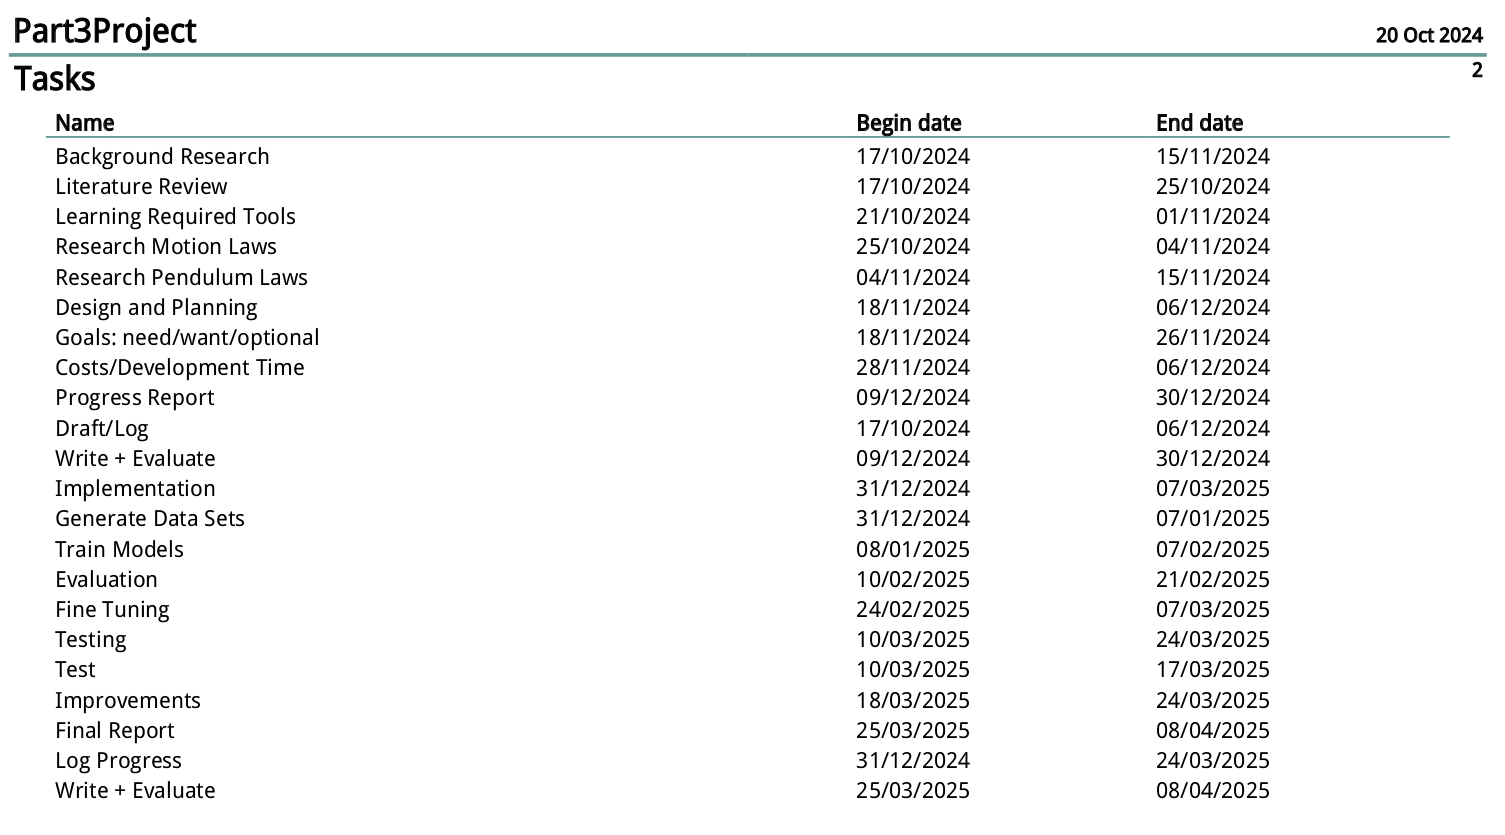
\includegraphics[width=16cm]{Gannt_Chart_Tasks}


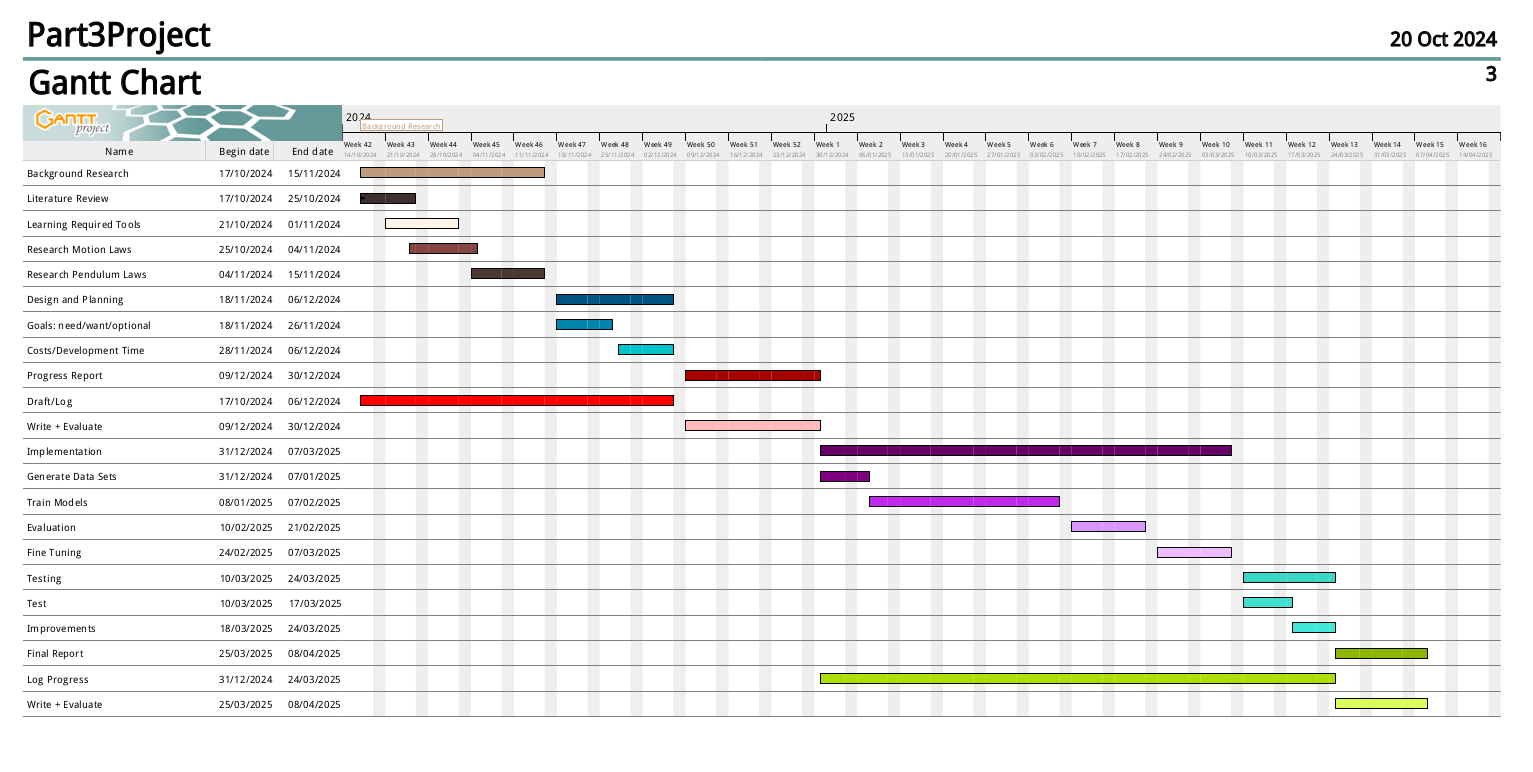
\includegraphics[width=15cm]{Gantt_Chart}

\section{Bibliography: }

[1] C. Wood Powerful ‘Machine Scientists’ Distill the Laws of Physics From Raw Data. Quanta Magazine, 2022.\\ 

[2] M. Schmidt and H. Lipson, Distilling Free-Form Natural Laws from Experimental Data. Science, 324, 5923,
2009.\\

[3] A. Koyr´e, The Astronomical Revolution: Copernicus-
Kepler-Borelli (Routledge, 2013).\\ 

[4] A Computational Inflection for Scientific Discovery by Hope, Tom and Downey, Doug and Weld, Daniel S. and Etzioni, Oren and Horvitz, Eric\\

[5] Schmidt M, Lipson H (2009) Distilling free-form natural laws from experimental data. Science
324(5923):81–85. \\

[6] Interpretability in symbolic regression: a benchmark of explanatory methods using the Feynman data set, Aldeia, Guilherme Seidyo Imai and de França, Fabrício Olivetti, 2022 \\ 

[7] "Discovering Symbolic Models from Deep Learning with Inductive Biases" by Miles Cranmer et al. (2020)\\ 

[8] "Scaling Up Symbolic Regression with Operator Grammars" by Michael O'Neill et al. (2020)\\ 

[9] "A Survey of Symbolic Regression Methods" by Bogdan Burlacu et al. (2020)\\ 

[10] "Regularized Evolution for Symbolic Regression" by Nguyen Quang Uy et al. (2011) \\ 

[11] Calculus: Early Transcendentals" by James Stewart\\ 

[12] Partial Differential Equations for Scientists and Engineers" by Stanley J. Farlow:\\ 

[13] A first course in Dimensional Analysis by Juan G Santiago\\ 

[14] W. Blasiak, M. Godlewska, R. Rosiek, and D. Wcislo, “Spectrum of
physics comprehension,” European Journal of Physics, vol. 33, p. 565,
2012. [Online]. Available: https://www.researchgate.net/publication/
254496494 Spectrum of physics comprehension\\

[15] K. S. Taber, “Maths should be the last thing we teach,” Physics
Education, vol. 44, no. 4, p. 336, jul 2009. [Online]. Available:
https://dx.doi.org/10.1088/0031-9120/44/4/F01\\ 

[16] Y. Zhu, Z. -Y. Khoo, J. S. Choong Low and S. Bressan, "A Personalised Learning Tool for Physics Undergraduate Students Built On a Large Language Model for Symbolic Regression," 2024 IEEE Conference on Artificial Intelligence (CAI), Singapore, Singapore, 2024, pp. 38-43, doi: 10.1109/CAI59869.2024.00017. keywords: {Knowledge engineering;Systematics;Large language models;Learning (artificial intelligence);Mathematical models;Physics education;Problem-solving;AI and Education;Symbolic Regression;Large Language Models;Physics Education;Prompt Engineering;Undergraduate Learning},\\

[17]  A Murari et al 2015 Plasma Phys. Control. Fusion 57 014008\\

[18]  Schmid M and Lipson H 2009 Science 324 81–5\\ 

[19] Koza J R 1992 Genetic Programming: On the Programming
of Computers by Means of Natural Selection (Cambridge,
MA: MIT Press)\\

[20] Burnham K P and Anderson D R 2002 Model Selection and
Multi-Model Inference: A Practical Information-Theoretic
Approach 2nd edn (Berlin: Springer)\\ 

[21] Fundementals of Dimensional Analysis Theory and Applications in Metallurgy, Alberto N.Conejo Springer\\ 

[22] Partial Derivatives Peter Hilton\\
\end{document}
